The Cypress CX3 is a MIPI to USB interface. This controller is fully functional with any image sensor that is compliant with a MIPI Camera Serial Interface (OmniVision 5640). The Cypress CX3 is used to control the communication between a computer and the device, since it uses a USB connection to power the device and transfer the data that it collected. Also in order for the device to store the data read from the camera module, it uses EEPROMS in order to prevent loosing data in cases the device looses power. Then the device will transfer its data to the computer via USB. The Cypress CX3 is also connected to the MIPI camera.
\begin{figure}[h!]
	\centering
 	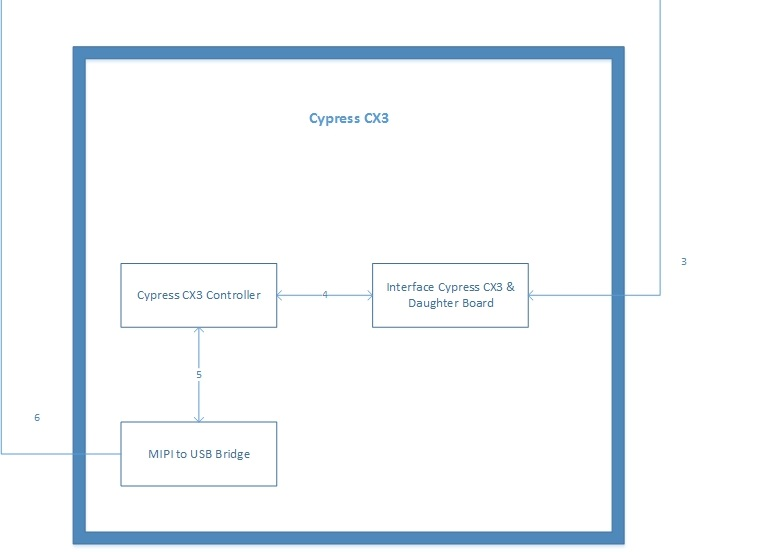
\includegraphics[width=0.60\textwidth]{images/Cypress}
 \caption{Cypress Subsystem Diagram}
\end{figure}



\subsection{Interface Cypress CX3 & Daughter Board}
This connector is used to interface between the daughter board and the CX3 Controller. The connector is also connected to the EEPROM of the device, since it will transfer the data collected and store it at the EEPROM. Other pins of the MIPI Camera BRD Connector are connected to CX3 Controller and the Base BRD Connector.

\begin{figure}[h!]
	\centering
 	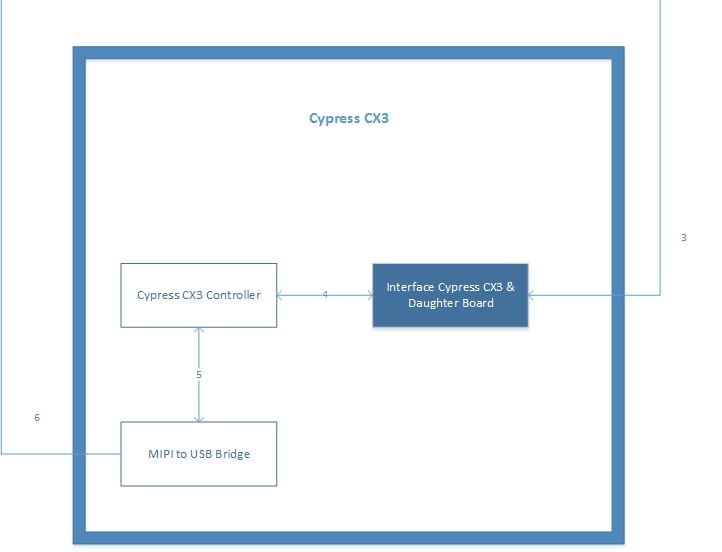
\includegraphics[width=0.60\textwidth]{images/Cypress_Interface}
 \caption{CX3 Daughter Board Interface Diagram}
\end{figure}

\subsubsection{Assumptions}
TBD

\subsubsection{Responsibilities}
TBD

\subsubsection{Subsystem Interfaces}

\begin {table}[H]
\caption {CX3- Daugther Board interface}
\begin{center}
    \begin{tabular}{ | p{1cm} | p{6cm} | p{3cm} | p{3cm} |}
    \hline
    ID & Description & Inputs & Outputs \\ \hline
    \#03 & Communication with Daughter Board & \pbox{3cm}{Input 1 - MIPI Data \\ Input 2 - MIPI Clock \\ Input 3 - MIPI Power \\ Input 4 - SDA} & \pbox{3cm}{Output 1 - SCL \\ Output 2 - SDA}  \\ \hline
    \end{tabular}
\end{center}
\end{table}

\subsection{Cypress CX3 Controller}
The main purpose of the CX3 Controller is to interface with the MIPI camera and then transfer the data collected to the CX3 USB interface. The CX3 Controller its also connected to multiple components of the Cypress CX3, but at the moment we have not determined which components will be needed for the Eye Tracker System. For example, we believe that the Eye Tracker System will not need to be connected to JTAG, so those pins on the controller will not be used.

\begin{figure}[h!]
	\centering
 	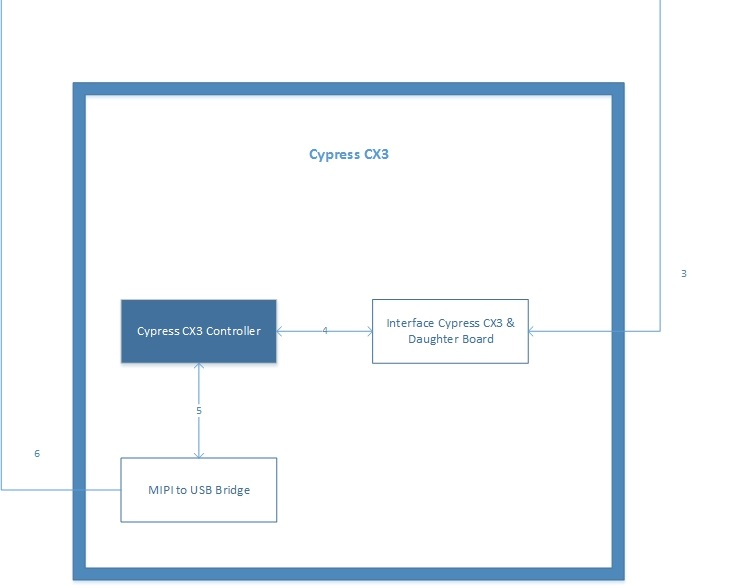
\includegraphics[width=0.60\textwidth]{images/Cypress_Controller}
 \caption{Cypress CX3 Controller interface}
\end{figure}

\subsubsection{Assumptions}
TBD

\subsubsection{Responsibilities}
TBD

\subsubsection{Subsystem Interfaces}
TBD

\begin {table}[H]
\caption {Cypress Cx3 Controller interface}
\begin{center}
    \begin{tabular}{ | p{1cm} | p{6cm} | p{3cm} | p{3cm} |}
    \hline
    ID & Description & Inputs & Outputs \\ \hline
    \#04 & Communication between CX3 Controller and MIPI & \pbox{3cm}{Input 1 - MIPI Data \\ Input 2 - MIPI Clock \\ Input 3 - MIPI Power \\ Input 4 - SDA} & \pbox{3cm}{Output 1 - SCL \\ Output 2 - SDA}  \\ \hline
    \#05 & Communication between CX3 Controller and USB Interface & \pbox{3cm}{Input 1 - SCL \\ Input 2 - SDA} & \pbox{3cm}{Output 1 - MIPI Clock \\ Output 2 - MIPI Data}  \\ \hline
    \end{tabular}
\end{center}
\end{table}

\subsection{MIPI to USB Bridge}
The main purpose of the CX3 USB Interface is to serve as a bridge connection of MIPI camera to USB. The entire system will be powered using the USB connection. This part of the CX3 is also connected to the CX3 Controller and transfers the data collected from the MIPI Camera to a computer via USB. Since this device transfers numerous amounts of data between the CX3 and the MIPI camera, it contains multiple internal clocks.

\begin{figure}[h!]
	\centering
 	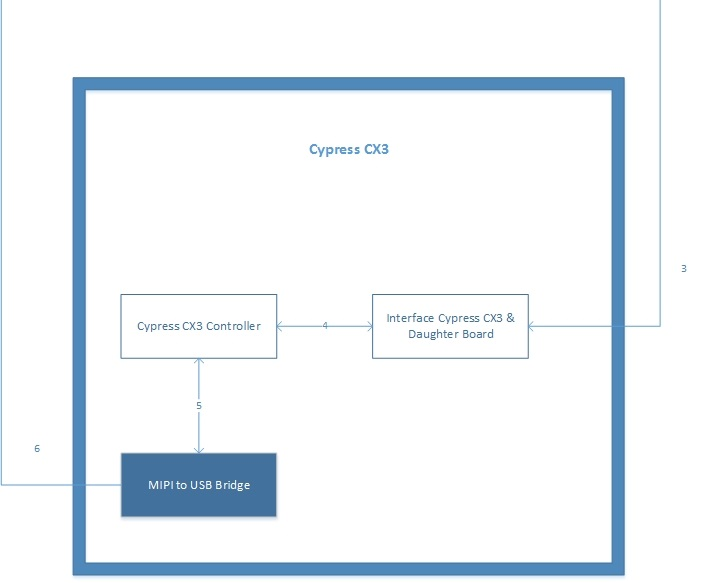
\includegraphics[width=0.60\textwidth]{images/Cypress_MIPI}
 \caption{MIPI to USB Subsystem}
\end{figure}

\subsubsection{Assumptions}
TBD

\subsubsection{Responsibilities}
TBD

\subsubsection{Subsystem Interfaces}
TBD

\begin {table}[H]
\caption {MIPI to USB interface}
\begin{center}
    \begin{tabular}{ | p{1cm} | p{6cm} | p{3cm} | p{3cm} |}
    \hline
    ID & Description & Inputs & Outputs \\ \hline
    \#05 & Communication between USB Interface and CX3 Controller & \pbox{3cm}{Input 1 - MIPI Clock \\ Input 2 - MIPI Data \\ Input 3 - CX3_GPIO} & \pbox{3cm}{Output 1 - SDA \\ Output 2 - SCL}  \\ \hline
    \#06 & Communication between USB Interface and Computer & \pbox{3cm}{N/A} & \pbox{3cm}{Output 1 - USB Data}  \\ \hline
    \end{tabular}
\end{center}
\end{table}
